\documentclass{beamer}


\usepackage[french,english]{babel}

\usepackage[T1]{fontenc}

\usepackage[utf8]{inputenc}
\usepackage[linesnumbered,ruled,vlined]{algorithm2e}

\usetheme{Warsaw}
\title{Apprentissage et résultats}

\author{Clément Legrand}

\begin{document}


\begin{frame}[plain]
\titlepage
\end{frame}

\section{Apprentissage}

\subsection{Description}

\begin{frame}{Description}
\begin{block}{Base de départ}
Les solutions données par CW.
\begin{itemize}
\item Tirage au sort de N triplets ($\lambda$, $\mu$, $\nu$);
\item Calcul des solutions pour tout triplet ($\lambda$, $\mu$, $\nu$).
\end{itemize}
\end{block}

\begin{block}{Base d'apprentissage}
On peut ne garder qu'une partie de la base générée pour apprendre
\begin{itemize}
\item On garde $x\%$ des meilleures solutions (quantité privilégiée, Quan$_{x}$);
\item On garde les solutions qui ont un coût inférieur à $c_{min} + (c_{max}-c_{min})\frac{x}{100}$ (qualité privilégiée, Qual$_{x}$).
\item On choisit d'utiliser toute la base générée pour apprendre (Tout)
\end{itemize}
\end{block}
\end{frame}

\begin{frame}{Protocole}

\begin{exampleblock}{Protocole}
\begin{itemize}
\item Génération de la base de départ
\item Calcul de la base d'apprentissage
\item On initialise une matrice MAT de taille $n^2$
\item Pour chaque arête (a,b) on incrémente la valeur MAT[a][b] (si a>b, on commence par échanger a et b)
\item Comparaison arêtes obtenues et optimales.
\end{itemize}
\end{exampleblock}

\begin{block}{Choix des arêtes}
\begin{itemize}
\item On conserve (a,b) si MAT[a][b] dépasse une certaine valeur (Seuil);
\item On conserve les k premières arêtes en triant selon les valeurs contenues dans MAT (Rang).
\end{itemize}
\end{block}

\end{frame}

\subsection{Résultats A-n37-k06}

\begin{frame}{Instance test}
3 instances ont été choisies pour réaliser ces tests: A-n37-k06, A-n65-k09 et P-n101-k04.

La solution employée pour comparer les résultats est celle de la littérature.

La meilleure solution comporte 42 arêtes.

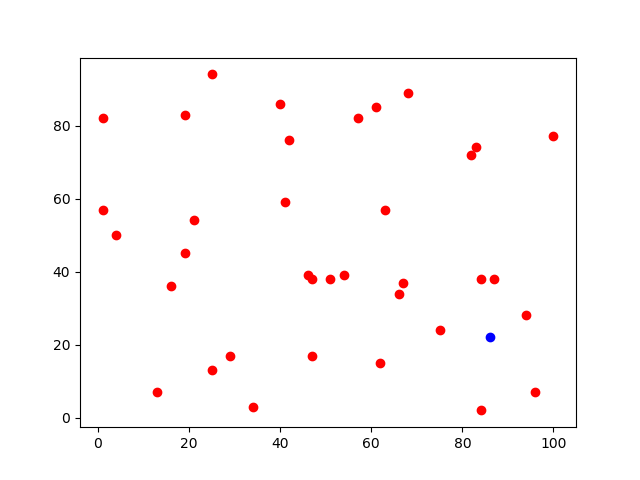
\includegraphics[scale=0.3]{instance3706.png}
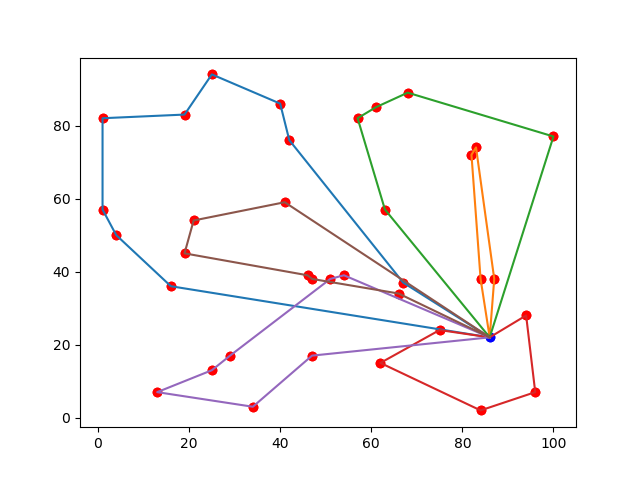
\includegraphics[scale=0.3]{best3706.png}

Pour chaque test on effectue 5 itérations.

Temps de calcul: 2 s (50), 4 s (100), 20 s (500), 44 s (1000).
\end{frame}

\begin{frame}{Résultats avec critère Seuil et base Quan$_{10}$}
\emph{L$_{lb}$} est la taille de la base d'apprentissage. 

On utilise la base Quan$_{10}$ avec certaines valeurs de seuil.

\begin{tabular}{|c|c|c|c|c|}
   \hline
   Taille base & Seuil & Nb arêtes & Nb correctes & Proportion\\
   \hline
   50 & L$_{lb}$/2 & 34 & 21 & 0.5  \\   
   \hline
   100 & L$_{lb}$/2 & 30 & 21 & 0.5  \\
   \hline
   500 & L$_{lb}$/2 & 32 & 24 & 0.57  \\
   \hline
   1000 & L$_{lb}$/2 & 33 & 24 & 0.57  \\
   \hline
   \hline
   50 & 3L$_{lb}$/4 & 23 & 14 & 0.33  \\
   \hline
   100 & 3L$_{lb}$/4 & 16 & 15 & 0.36  \\
   \hline
   500 & 3L$_{lb}$/4 & 15 & 14 & 0.33  \\
   \hline
   1000 & 3L$_{lb}$/4 & 16 & 14 & 0.33  \\
   \hline
\end{tabular}


\end{frame}

\begin{frame}{Résultats avec critère Seuil et base Qual$_{10}$}
On utilise la base Qual$_{10}$ avec certaines valeurs de seuil.
\begin{tabular}{|c|c|c|c|c|}
   \hline
   Taille base & Seuil & Nb arêtes & Nb correctes & Proportion\\
    \hline
   50 & L$_{lb}$/2 & 33 & 21 & 0.50  \\
   \hline
   100 & L$_{lb}$/2 & 31 & 23 & 0.55  \\
   \hline
   500 & L$_{lb}$/2 & 31 & 22 & 0.52  \\
   \hline
   1000 & L$_{lb}$/2 & 31 & 23 & 0.53  \\
   \hline
   \hline
   50 & 3L$_{lb}$/4 & 17 & 12 & 0.28  \\
   \hline
   100 & 3L$_{lb}$/4 & 17 & 14 & 0.33  \\
   \hline
   500 & 3L$_{lb}$/4 & 20 & 16 & 0.38  \\
   \hline
   1000 & 3L$_{lb}$/4 & 19 & 16 & 0.38  \\
   \hline
\end{tabular}
\end{frame}

\begin{frame}{Résultats avec critère Seuil et base Tout}
On utilise la base Tout avec certaines valeurs de seuil.
\begin{tabular}{|c|c|c|c|c|}
   \hline
   Taille base & Seuil & Nb arêtes & Nb correctes & Proportion\\
   \hline
   50 & L$_{lb}$/2 & 23 & 15 & 0.35  \\
   \hline
   100 & L$_{lb}$/2 & 24 & 17 & 0.40  \\
   \hline
   500 & L$_{lb}$/2 & 22 & 15 & 0.36  \\
   \hline
   1000 & L$_{lb}$/2 & 23 & 16 & 0.38  \\
   \hline
   \hline
   50 & 3L$_{lb}$/4 & 10 & 7 & 0.16  \\
   \hline
   100 & 3L$_{lb}$/4 & 6 & 6 & 0.14  \\
   \hline
   500 & 3L$_{lb}$/4 & 7 & 7 & 0.18  \\
   \hline
   1000 & 3L$_{lb}$/4 & 6 & 6 & 0.14  \\
   \hline
\end{tabular}
\end{frame}


\begin{frame}{Résultats avec critère Rang et base Quan$_{10}$}

On utilise la base Quan$_{10}$ avec certaines valeurs de rang.
\begin{tabular}{|c|c|c|c|}
   \hline
   Taille base & Rang max & Nb correctes & Proportion\\
   \hline
   50 & 10  & 6 & 0.14  \\
   \hline
   100 & 10  & 9 & 0.21  \\
   \hline
   500 & 10  & 9 & 0.21  \\
   \hline
   1000 & 10 & 9 & 0.21  \\
   \hline
   \hline
   50 & 20 & 13 & 0.31  \\
   \hline
   100 & 20 & 16 & 0.38  \\
   \hline
   500 & 20 & 16 & 0.38  \\
   \hline
   1000 & 20 & 17 & 0.40  \\
   \hline
   \hline
   50 & n/2 & 12 & 0.28  \\
   \hline
   100 & n/2 & 13 & 0.3  \\
   \hline
   500 & n/2 & 13 & 0.3  \\
   \hline
   1000 & n/2 & 13 & 0.3  \\
   \hline
\end{tabular}

\end{frame}

\begin{frame}{Résultats avec critère Rang et base Qual$_{10}$}

On utilise la base Qual$_{10}$ avec certaines valeurs de rang.
\begin{tabular}{|c|c|c|c|}
   \hline
   Taille base & Rang max & Nb correctes & Proportion\\
   \hline
   50 & 10  & 6 & 0.14  \\
   \hline
   100 & 10  & 9 & 0.21  \\
   \hline
   500 & 10  & 10 & 0.24  \\
   \hline
   1000 & 10 & 10 & 0.24  \\
   \hline
   \hline
   50 & 20  & 13 & 0.32  \\
   \hline
   100 & 20 & 16 & 0.38  \\
   \hline
   500 & 20 & 16 & 0.38  \\
   \hline
   1000 & 20 & 16 & 0.38  \\
   \hline
   \hline
   50 & n/2 & 13 & 0.3  \\
   \hline
   100 & n/2 & 13 & 0.3  \\
   \hline
   500 & n/2 & 13 & 0.3  \\
   \hline
   1000 & n/2 & 12 & 0.29  \\
   \hline
\end{tabular}
\end{frame}

\begin{frame}{Résultats avec critère Rang et base Tout}

On utilise la base Tout avec certaines valeurs de rang.
\begin{tabular}{|c|c|c|c|}
   \hline
   Taille base & Rang max & Nb correctes & Proportion\\
   \hline
   50 & 10  & 7 & 0.16  \\
   \hline
   100 & 10  & 10 & 0.24  \\
   \hline
   500 & 10  & 9 & 0.21  \\
   \hline
   1000 & 10 & 10 & 0.24  \\
   \hline
   \hline
   50 & 20  & 13 & 0.31  \\
   \hline
   100 & 20 & 15 & 0.36  \\
   \hline
   500 & 20 & 15 & 0.36  \\
   \hline
   1000 & 20 & 15 & 0.36  \\
   \hline
   \hline
   50 & n/2 & 12 & 0.28  \\
   \hline
   100 & n/2 & 12 & 0.29  \\
   \hline
   500 & n/2 & 12 & 0.28  \\
   \hline
   1000 & n/2 & 12 & 0.28  \\
   \hline
\end{tabular}
\end{frame}

\begin{frame}{Résultats avec toutes les SI}
Temps de calcul pour avoir la base : 37.5 s

\centering
\begin{tabular}{|c|c|c|c|}
   \hline
   Seuil & Rés Quan$_{10}$ & Rés Qual$_{10}$ & Tout \\
   \hline
   L$_{lb}$/2 & 33 - 24 - 0.57 & 30 - 23 - 0.55 & 25 - 16 - 0.38 \\
   \hline
   3L$_{lb}$/4 & 15 - 14 - 0.33 & 18 - 16 - 0.38  & 9 - 6 - 0.14 \\
   \hline
\end{tabular}

\begin{tabular}{|c|c|c|c|}
   \hline
   Rang max & Rés Quan$_{10}$ & Rés Qual$_{10}$ & Tout\\
   \hline
   10 & 8 - 0.19 & 9 - 0.21 & 7 - 0.17 \\
   \hline
   20 & 14 - 0.33 & 14 - 0.33 & 13 - 0.31\\
   \hline
   n/2 & 12 - 0.29 & 12 - 0.29 & 12 - 0.29 \\
   \hline
\end{tabular}

\end{frame}

\subsection{Résultats A-n65-k09}

\begin{frame}{Instance test}

La solution employée pour comparer les résultats est celle de la littérature.

La meilleure solution comporte 73 arêtes.

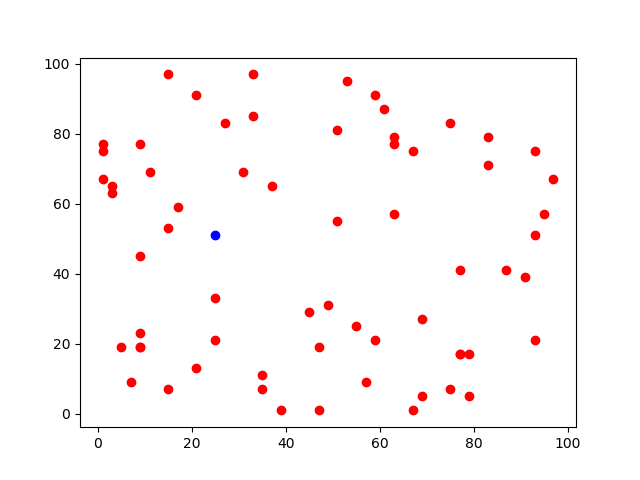
\includegraphics[scale=0.3]{Instance6509.png}
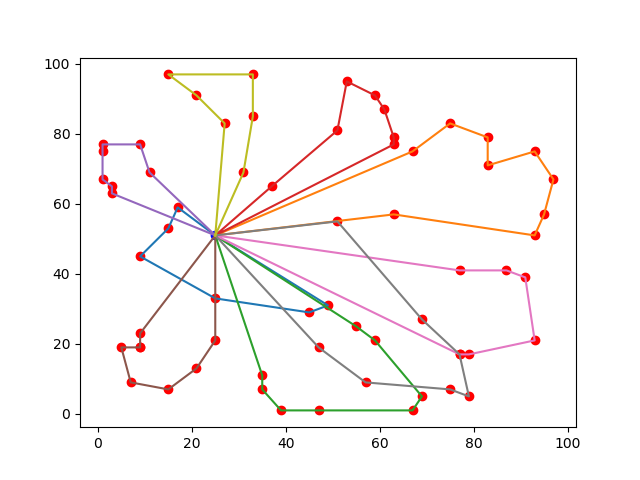
\includegraphics[scale=0.3]{Solution6509.png}

Pour chaque test on effectue 5 itérations.

Temps de calcul: 4 s (50), 8 s (100), 42 s (500), 84 s (1000).
\end{frame}

\begin{frame}{Résultats avec critère Seuil et base Quan$_{10}$}
\emph{L$_{lb}$} est la taille de la base d'apprentissage. 


On utilise la base Quan$_{10}$ avec certaines valeurs de seuil.

\begin{tabular}{|c|c|c|c|c|}
   \hline
   Taille base & Seuil & Nb arêtes & Nb correctes & Proportion\\
   \hline
   50 & L$_{lb}$/2 & 73 & 43 & 0.59  \\   
   \hline
   100 & L$_{lb}$/2 & 70 & 44 & 0.6  \\
   \hline
   500 & L$_{lb}$/2 & 71 & 43 & 0.59  \\
   \hline
   1000 & L$_{lb}$/2 & 71 & 43 & 0.59  \\
   \hline
   \hline
   50 & 3L$_{lb}$/4 & 61 & 40 & 0.55  \\
   \hline
   100 & 3L$_{lb}$/4 & 63 & 41 & 0.56  \\
   \hline
   500 & 3L$_{lb}$/4 & 60 & 40 & 0.55  \\
   \hline
   1000 & 3L$_{lb}$/4 & 57 & 40 & 0.54  \\
   \hline
\end{tabular}


\end{frame}

\begin{frame}{Résultats avec critère Seuil et base Qual$_{10}$}
On utilise la base Qual$_{10}$ avec certaines valeurs de seuil.
\begin{tabular}{|c|c|c|c|c|}
   \hline
   Taille base & Seuil & Nb arêtes & Nb correctes & Proportion\\
    \hline
   50 & L$_{lb}$/2 & 64 & 44 & 0.60  \\
   \hline
   100 & L$_{lb}$/2 & 58 & 42 & 0.58  \\
   \hline
   500 & L$_{lb}$/2 & 56 & 41 & 0.56  \\
   \hline
   1000 & L$_{lb}$/2 & 55 & 41 & 0.56  \\
   \hline
   \hline
   50 & 3L$_{lb}$/4 & 39 & 29 & 0.40  \\
   \hline
   100 & 3L$_{lb}$/4 & 36 & 28 & 0.39  \\
   \hline
   500 & 3L$_{lb}$/4 & 35 & 28 & 0.39  \\
   \hline
   1000 & 3L$_{lb}$/4 & 35 & 27 & 0.38  \\
   \hline
\end{tabular}
\end{frame}

\begin{frame}{Résultats avec critère Seuil et base Tout}
On utilise la base Tout avec certaines valeurs de seuil.
\begin{tabular}{|c|c|c|c|c|}
   \hline
   Taille base & Seuil & Nb arêtes & Nb correctes & Proportion\\
   \hline
   50 & L$_{lb}$/2 & 40 & 31 & 0.43  \\
   \hline
   100 & L$_{lb}$/2 & 43 & 33 & 0.45  \\
   \hline
   500 & L$_{lb}$/2 & 45 & 35 & 0.48  \\
   \hline
   1000 & L$_{lb}$/2 & 45 & 35 & 0.48  \\
   \hline
   \hline
   50 & 3L$_{lb}$/4 & 14 & 9 & 0.13  \\
   \hline
   100 & 3L$_{lb}$/4 & 15 & 10 & 0.14  \\
   \hline
   500 & 3L$_{lb}$/4 & 14 & 9 & 0.13  \\
   \hline
   1000 & 3L$_{lb}$/4 & 13 & 9 & 0.13  \\
   \hline
\end{tabular}
\end{frame}


\begin{frame}{Résultats avec critère Rang et base Quan$_{10}$}

On utilise la base Quan$_{10}$ avec certaines valeurs de rang.
\begin{tabular}{|c|c|c|c|}
   \hline
   Taille base & Rang max & Nb correctes & Proportion\\
   \hline
   50 & 10  & 6 & 0.08  \\
   \hline
   100 & 10  & 6 & 0.08  \\
   \hline
   500 & 10  & 7 & 0.1  \\
   \hline
   1000 & 10 & 7 & 0.1  \\
   \hline
   \hline
   50 & 20 & 14 & 0.2  \\
   \hline
   100 & 20 & 16 & 0.22  \\
   \hline
   500 & 20 & 17 & 0.23  \\
   \hline
   1000 & 20 & 17 & 0.23  \\
   \hline
   \hline
   50 & n/2 & 23 & 0.32  \\
   \hline
   100 & n/2 & 26 & 0.36  \\
   \hline
   500 & n/2 & 27 & 0.36  \\
   \hline
   1000 & n/2 & 26 & 0.36  \\
   \hline
\end{tabular}

\end{frame}

\begin{frame}{Résultats avec critère Rang et base Qual$_{10}$}

On utilise la base Qual$_{10}$ avec certaines valeurs de rang.
\begin{tabular}{|c|c|c|c|}
   \hline
   Taille base & Rang max & Nb correctes & Proportion\\
   \hline
   50 & 10  & 7 & 0.1  \\
   \hline
   100 & 10  & 7 & 0.1  \\
   \hline
   500 & 10  & 7 & 0.1  \\
   \hline
   1000 & 10 & 7 & 0.1  \\
   \hline
   \hline
   50 & 20  & 15 & 0.21  \\
   \hline
   100 & 20 & 16 & 0.22  \\
   \hline
   500 & 20 & 15 & 0.21  \\
   \hline
   1000 & 20 & 15 & 0.21  \\
   \hline
   \hline
   50 & n/2 & 26 & 0.36  \\
   \hline
   100 & n/2 & 26 & 0.36  \\
   \hline
   500 & n/2 & 26 & 0.36  \\
   \hline
   1000 & n/2 & 26 & 0.36  \\
   \hline
\end{tabular}
\end{frame}

\begin{frame}{Résultats avec critère Rang et base Tout}

On utilise la base Tout avec certaines valeurs de rang.
\begin{tabular}{|c|c|c|c|}
   \hline
   Taille base & Rang max & Nb correctes & Proportion\\
   \hline
   50 & 10  & 7 & 0.1  \\
   \hline
   100 & 10  & 7 & 0.1  \\
   \hline
   500 & 10  & 6 & 0.08  \\
   \hline
   1000 & 10 & 6 & 0.08  \\
   \hline
   \hline
   50 & 20  & 14 & 0.19  \\
   \hline
   100 & 20 & 14 & 0.19  \\
   \hline
   500 & 20 & 13 & 0.18  \\
   \hline
   1000 & 20 & 13 & 0.18  \\
   \hline
   \hline
   50 & n/2 & 24 & 0.33  \\
   \hline
   100 & n/2 & 25 & 0.34  \\
   \hline
   500 & n/2 & 25 & 0.34  \\
   \hline
   1000 & n/2 & 25 & 0.34  \\
   \hline
\end{tabular}
\end{frame}


\begin{frame}{Résultats avec toutes les SI}
Temps de calcul pour avoir la base : 110 s

\centering
\begin{tabular}{|c|c|c|c|}
   \hline
   Seuil & Rés Quan$_{10}$ & Rés Qual$_{10}$ & Tout \\
   \hline
   L$_{lb}$/2 & 73 - 45 - 0.62 & 56 - 40 - 0.55 & 45 - 35 - 0.48 \\
   \hline
   3L$_{lb}$/4 & 62 - 41 - 0.56 & 35 - 28 - 0.38  & 13 - 9 - 0.12 \\
   \hline
\end{tabular}

\begin{tabular}{|c|c|c|c|}
   \hline
   Rang max & Rés Quan$_{10}$ & Rés Qual$_{10}$ & Tout \\
   \hline
   10 & 7 - 0.1 & 7 - 0.1 & 6 - 0.08 \\
   \hline
   20 & 17 - 0.23 & 17 - 0.23 & 13 - 0.18 \\
   \hline
   n/2 & 27 - 0.37 & 27 - 0.37 & 25 - 0.34 \\
   \hline
\end{tabular}

\end{frame}


\subsection{Résultats P-n101-k04}

\begin{frame}{Instance test}

La solution employée pour comparer les résultats est celle de la littérature.

La meilleure solution comporte 104 arêtes.

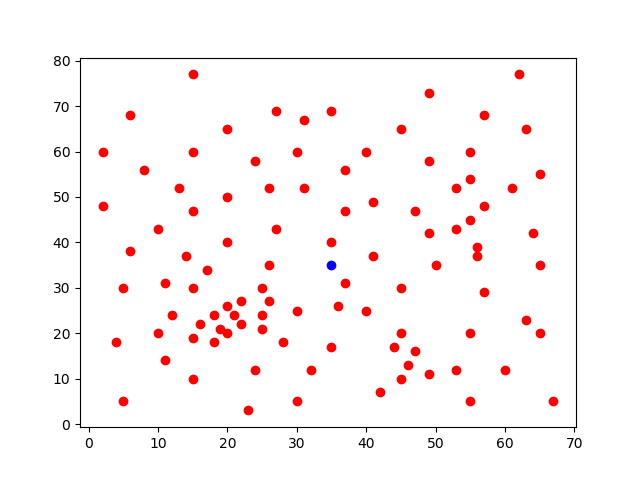
\includegraphics[scale=0.3]{Instance10104.png}
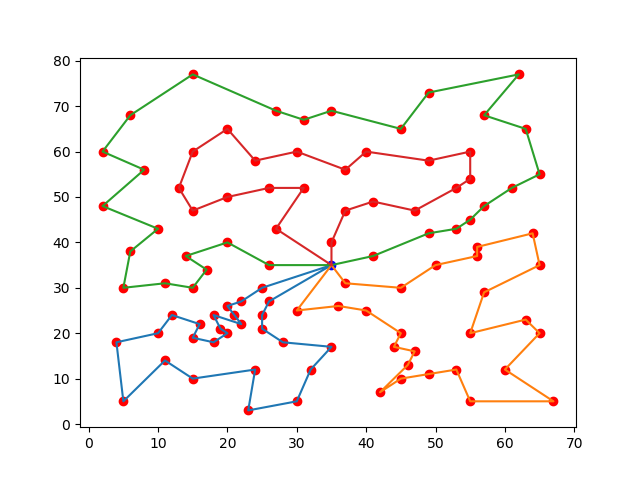
\includegraphics[scale=0.3]{Solution10104.png}

Pour chaque test on effectue 5 itérations.

Temps de calcul: 38 s (50), 75 s (100), 375 s (500). 
\end{frame}

\begin{frame}{Résultats avec critère Seuil et base Quan$_{10}$}
\emph{L$_{lb}$} est la taille de la base d'apprentissage. 


On utilise la base Quan$_{10}$ avec certaines valeurs de seuil.

\begin{tabular}{|c|c|c|c|c|}
   \hline
   Taille base & Seuil & Nb arêtes & Nb correctes & Proportion\\
   \hline
   50 & L$_{lb}$/2 & 93 & 65 & 0.62  \\   
   \hline
   100 & L$_{lb}$/2 & 80 & 66 & 0.64  \\
   \hline
   500 & L$_{lb}$/2 & 83 & 69 & 0.67  \\
   \hline
   \hline
   50 & 3L$_{lb}$/4 & 54 & 44 & 0.42  \\
   \hline
   100 & 3L$_{lb}$/4 & 45 & 41 & 0.39  \\
   \hline
   500 & 3L$_{lb}$/4 & 43 & 39 & 0.37  \\
   \hline
\end{tabular}


\end{frame}

\begin{frame}{Résultats avec critère Seuil et base Qual$_{10}$}
On utilise la base Qual$_{10}$ avec certaines valeurs de seuil.
\begin{tabular}{|c|c|c|c|c|}
   \hline
   Taille base & Seuil & Nb arêtes & Nb correctes & Proportion\\
    \hline
   50 & L$_{lb}$/2 & 83 & 66 & 0.64  \\
   \hline
   100 & L$_{lb}$/2 & 79 & 66 & 0.63  \\
   \hline
   500 & L$_{lb}$/2 & 81 & 68 & 0.66  \\
   \hline
   \hline
   50 & 3L$_{lb}$/4 & 42 & 37 & 0.36  \\
   \hline
   100 & 3L$_{lb}$/4 & 42 & 39 & 0.37  \\
   \hline
   500 & 3L$_{lb}$/4 & 39 & 36 & 0.35  \\
   \hline
\end{tabular}
\end{frame}

\begin{frame}{Résultats avec critère Seuil et base Tout}
On utilise la base Tout avec certaines valeurs de seuil.
\begin{tabular}{|c|c|c|c|c|}
   \hline
   Taille base & Seuil & Nb arêtes & Nb correctes & Proportion\\
   \hline
   50 & L$_{lb}$/2 & 71 & 61 & 0.59  \\
   \hline
   100 & L$_{lb}$/2 & 72 & 62 & 0.60  \\
   \hline
   500 & L$_{lb}$/2 & 72 & 63 & 0.60  \\
   \hline
   \hline
   50 & 3L$_{lb}$/4 & 24 & 21 & 0.20  \\
   \hline
   100 & 3L$_{lb}$/4 & 24 & 22 & 0.21  \\
   \hline
   500 & 3L$_{lb}$/4 & 22 & 20 & 0.19  \\
   \hline
\end{tabular}
\end{frame}


\begin{frame}{Résultats avec critère Rang et base Quan$_{10}$}

On utilise la base Quan$_{10}$ avec certaines valeurs de rang.
\begin{tabular}{|c|c|c|c|}
   \hline
   Taille base & Rang max & Nb correctes & Proportion\\
   \hline
   50 & 10  & 8 & 0.08  \\
   \hline
   100 & 10  & 8 & 0.08  \\
   \hline
   500 & 10  & 8 & 0.08  \\
   \hline
   \hline
   50 & 20 & 18 & 0.17  \\
   \hline
   100 & 20 & 18 & 0.17  \\
   \hline
   500 & 20 & 18 & 0.17  \\
   \hline
   \hline
   50 & n/2 & 43 & 0.41  \\
   \hline
   100 & n/2 & 45 & 0.43  \\
   \hline
   500 & n/2 & 46 & 0.44  \\
   \hline
\end{tabular}

\end{frame}

\begin{frame}{Résultats avec critère Rang et base Qual$_{10}$}

On utilise la base Qual$_{10}$ avec certaines valeurs de rang.
\begin{tabular}{|c|c|c|c|}
   \hline
   Taille base & Rang max & Nb correctes & Proportion\\
   \hline
   50 & 10  & 8 & 0.08  \\
   \hline
   100 & 10  & 8 & 0.08  \\
   \hline
   500 & 10  & 8 & 0.08  \\
   \hline
   \hline
   50 & 20  & 17 & 0.16  \\
   \hline
   100 & 20 & 18 & 0.17  \\
   \hline
   500 & 20 & 18 & 0.17  \\
   \hline
   \hline
   50 & n/2 & 44 & 0.43  \\
   \hline
   100 & n/2 & 45 & 0.43  \\
   \hline
   500 & n/2 & 46 & 0.44  \\
   \hline
\end{tabular}
\end{frame}

\begin{frame}{Résultats avec critère Rang et base Tout}

On utilise la base Tout avec certaines valeurs de rang.
\begin{tabular}{|c|c|c|c|}
   \hline
   Taille base & Rang max & Nb correctes & Proportion\\
   \hline
   50 & 10  & 8 & 0.08  \\
   \hline
   100 & 10  & 8 & 0.08  \\
   \hline
   500 & 10  & 8 & 0.08  \\
   \hline
   \hline
   50 & 20  & 18 & 0.17  \\
   \hline
   100 & 20 & 18 & 0.17  \\
   \hline
   500 & 20 & 18 & 0.17  \\
   \hline
   \hline
   50 & n/2 & 44 & 0.43  \\
   \hline
   100 & n/2 & 46 & 0.44  \\
   \hline
   500 & n/2 & 46 & 0.44  \\
   \hline
\end{tabular}
\end{frame}


\begin{frame}{Résultats avec toutes les SI}
Temps de calcul pour avoir la base : 1060 s

\centering
\begin{tabular}{|c|c|c|c|}
   \hline
   Seuil & Rés Quan$_{10}$ & Rés Qual$_{10}$ & Tout \\
   \hline
   L$_{lb}$/2 & 87 - 73 - 0.7 & 85 - 71 - 0.68 & 70 - 60 - 0.58 \\
   \hline
   3L$_{lb}$/4 & 42 - 39 - 0.38 & 41 - 38 - 0.37  & 23 - 21 - 0.2 \\
   \hline
\end{tabular}

\begin{tabular}{|c|c|c|c|}
   \hline
   Rang max & Rés Quan$_{10}$ & Rés Qual$_{10}$ & Tout \\
   \hline
   10 & 8 - 0.08 & 8 - 0.08 & 8 - 0.08 \\
   \hline
   20 & 18 - 0.17 & 18 - 0.17 & 18 - 0.17 \\
   \hline
   n/2 & 46 - 0.44 & 46 - 0.44 & 46 - 0.44 \\
   \hline
\end{tabular}

\end{frame}

\section{Intégration de la connaissance dans un algorithme}

\subsection{Présentation algorithme}
\begin{frame}{Algorithme actuel}

\begin{algorithm}[H]
\DontPrintSemicolon % Some LaTeX compilers require you to use \dontprintsemicolon instead
Déterminer $Init$ par apprentissage\;
$newBase \gets []$\;
\For {$i \gets 1$ \textbf{to} $10$} {
	$(\lambda,\mu,\nu) \gets argmin_{(\lambda,\mu,\nu)}CW(I,D,\lambda,\mu,\nu)$\;
	\If {$i = 1$} {
		$Sol \gets Heuristique(Init,I,D,\lambda,\mu,\nu)$\;
		$newBase \gets newBase \cup Sol$\;
	}
	\Else {
		Déterminer $Init$ avec les connaissances de $Base$\;
		 $Sol \gets Heuristique(Init,I,D,\lambda,\mu,\nu)$\;
		$newBase \gets newBase \cup Sol$\;
	}
}
\Return{La meilleure solution}\;

\end{algorithm}

\end{frame}

\subsection{Résultats}

\begin{frame}{Premiers résultats}
\begin{block}{Choix}
Pour extraire les connaissances, je prends :
\begin{itemize}
\item Base : Qual$_{10}$
\item Critère : Rang = n/2
\end{itemize}
\end{block}

Résultats pour les coûts obtenus
\begin{tabular}{|c|c|c|c|}
   \hline
   Méthode  & A-n37-k06 (952) & A-n65-k09 (1182) & P-n101-k04 (692)  \\
   \hline
   Sans & 963 - 974  & 1189 - 1236 & 696 - 708   \\
   \hline
   Avec & 950 - 966 & 1186 - 1193 & 694 - 704  \\
   \hline
\end{tabular}

Résultats pour le temps d'exécution (en sec)
\begin{tabular}{|c|c|c|c|}
   \hline
   Méthode  & A-n37-k06 & A-n65-k09 & P-n101-k04  \\
   \hline
   Sans & 805  & 776 &  1739  \\
   \hline
   Avec & 3 - 1073 & 8 - 911 & 78 - 1533  \\
   \hline
\end{tabular}

\end{frame}

\begin{frame}{Nouveau meilleur résultat}
Pour l'instance Golden-01, nouvelle solution trouvée:

\begin{figure}
\centering
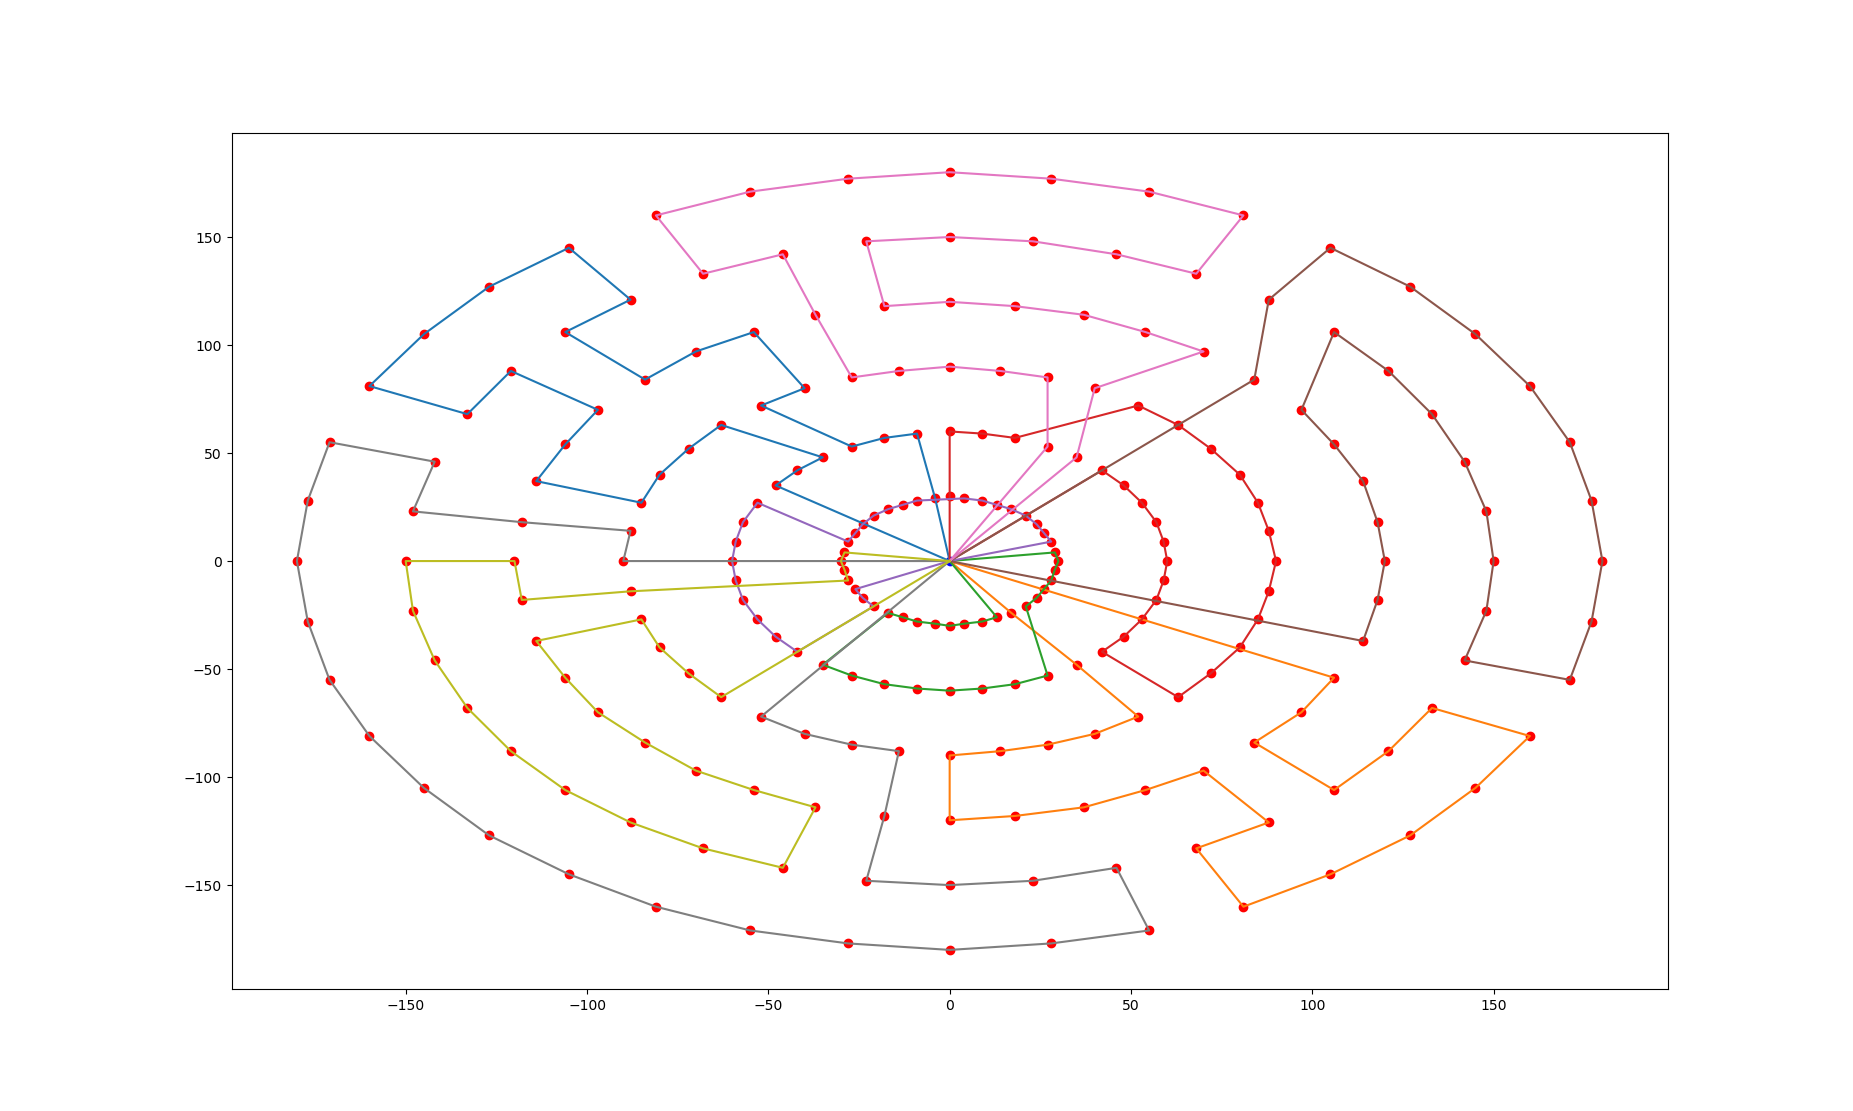
\includegraphics[scale=0.2]{NewBestG01}
\end{figure}

Coût de 5602 au lieu de 5623
\end{frame}

\end{document}
